\clearpage
\refstepcounter{PagePtr}\label{P:challenge}
\section{チャレンジ}
\begin{itemize}
  \item 例題、問題をすべて解こう
  \item 発表会に向けて、自分が作りたいプログラムを考えよう
  \begin{itemize}
    \item 今まで習ったセンサーやFabo、OpenJtalk、Julius、ゲーム、スクレイピング、CGIなど組み合わせられるか考えてみよう
    \item 自分の作りたいプログラムのアイデアを下のアイデアノートに書いておこう。今まで習ったサンプルプログラムで使えそうなのはあるかな?
  \end{itemize}
\end{itemize}
アイデアノート

\begin{center}
\tablefirsthead{}
\tablehead{}
\tabletail{}
\tablelasttail{}
\begin{boxedminipage}{16.806cm}
	                         
	\vspace{15cm}
\end{boxedminipage}
\end{center}

\clearpage
\section{付録 サンプルプログラムリスト}
授業では使用していない、サンプルプログラムのリストを上げておきます。
プログラムの解説はプログラムファイル内にのコメントとしてついています。
プログラムを開いて解説を読んでください。

\begin{flushleft}
\tablefirsthead{}
\tablehead{}
\tabletail{}
\tablelasttail{}
\begin{supertabular}{|m{6.7730002cm}|m{2.042cm}|m{7.5810003cm}|}
\hline
ファイルの場所 & 例題 & 機能説明\\\hline
\textbf{{\textasciitilde}/08/tv.hsp} & \ref*{E:TV} &
TVの番組表で検索をして次に放送される番組1つを取得して表示するプログラム。スクリプトエディタで読み込んで、F5で実行\\\hline
\textbf{{\textasciitilde}/08/weblio.hsp} & \ref*{E:Weblio} &
英単語を辞書で検索して、\ruby{日本語訳}{にほんごやく}を表示するプログラム。スクリプトエディタで読み込んで、F5で実行\\\hline
\textbf{{\textasciitilde}/08/eki.hsp} &\ref*{E:station} &
最寄り駅とその路線情報を取得して表示するプログラム。
スクリプトエディタで読み込んで、F5で実行\\\hline
\textbf{{\textasciitilde}/08/zipcode.hsp} & \ref*{E:postNum} &
郵便番号から住所を検索するプログラム。スクリプトエディタで読み込んで、F5で実行\\\hline
\textbf{{\textasciitilde}/08/wikipedia.hsp} & \ref*{E:wikipedia} &
ウィキペディアで用語を検索して、最初の数行を表示するプログラム。
スクリプトエディタで読み込んで、F5で実行\\\hline
\textbf{{\textasciitilde}/08/friend.hsp} & なし &
friend\_ipで指定したIPアドレスの友達のウェブページからランキングを取得して表示するプログラム。
スクリプトエディタで読み込んで、F5で実行\\\hline
\textbf{{\textasciitilde}/08/www/cgi-bin/ascii\_table.hsp} & なし &
ASCIIの表を取得して表示するプログラム。ウェブサーバを起動して

	\textbf{cd {\textasciitilde}/08/www}

	\textbf{./webserver.py}

ブラウザで

	\textbf{localhost:3000/cgi-bin/ascii\_table.hsp}

を開くすると表が表示されます。\\\hline
\textbf{{\textasciitilde}/08/www/ascii\_table.html} & なし &
上の例題プログラムが表示する表と全く同じもの。
ウェブサーバを立ち上げなくても、このファイルをブラウザで開くだけで表が表示できる。

ブラウザで

	\textbf{{\textasciitilde}/08/www/ascii\_table.html}

を開く\\\hline
\end{supertabular}
\end{flushleft}

\clearpage
\section{付録 HSPからスクレイピングをするときに便利な命令\ruby{一覧}{いちらん}}
\begin{center}
\tablefirsthead{}
\tablehead{}
\tabletail{}
\tablelasttail{}
\begin{supertabular}{|m{2.349cm}|m{7.57cm}|m{6.487cm}|}
\hline
命令名 & 書式 & 機能\\\hline
curl &
\#include “hspcurl.as”

curl “URL”, filename &
URLで指定されるデータをfilenameとして保存する\\\hline
creattmp &
\#include “htmlparser.as”

creattmp filename &
一時ファイルを作成する。作成したファイル名はfilenameに文字列として\ruby{渡}{わた}される\\\hline
deltmp &
\#include “htmlparser.as”

deltmp filename &
filenameで指定されるファイルを\ruby{削除}{さくじょ}する。
	プログラム内で作った、一時ファイルを削除するのに便利\\\hline
htmltag &
\#include “htmlparser.as”

htmltag buf1, “tag”, buf2 &
buf1内の”tag”を探して、buf2に書き出す\\\hline
htmltagn &
\#include “htmlparser.as”

1) htmltagn buf1, “tag”, 0, 1, buf2

~

2) htmltagn buf1, “tag”, 2, -1, buf2 &
1)
buf1内の”tag”を探して、0番目(1つめ)から、1つ分取り出してbuf2へ書き出す(1のタグ)

2)
buf1内の”tag”を探して、2番目(3つめ)から、すべて取り出してbuf2へ書き出す(3{\textasciitilde}すべてのタグ)\\\hline
htmltagattr &
\#include “htmlparser.as”

htmltagattr buf1, “tag”, “attr:val”, buf2 &
buf1内の”{\textless}tag
attr=val{\textgreater}”を探して、buf2へ書き出す\\\hline
htmltext &
\#include “htmlparser.as”

htmltext buf1, “tag”, buf2 &
buf1内の”tag”を探し{\textless}tag{\textgreater}{\textless}/tag{\textgreater}を取り除くいてbuf2に書き出す(タグの間にある文字列だけにする)\\\hline
htmluntag &
\#include “htmlparser.as”

htmluntag buf1, buf2 &
buf1内の{\textless}tag{\textgreater}{\textless}/tag{\textgreater}をすべて取り除くいてbuf2に書き出す(タグの間にある文字列だけにする)\\\hline
htmlval &
\#include “htmlparser.as”

htmlval buf1, “tag”, “attr”, buf2 &
buf1内の”tag”を探して,
“attr”に対応する値を取り出してbuf2へ書き出す({\textless}tag
attr=val{\textgreater}のval)\\\hline
htmltable &
\#include “htmlparser.as”

htmltable buf1, “attr:val”, buf2 &
buf1の{\textless}table
attr=val{\textgreater}を探してその中の{\textless}td{\textgreater}{\textless}/td{\textgreater}の間の文字列をbuf2へ入れる\\\hline
splitnl &
splitnl buf1, array &
buf1を改行を区切り文字として\ruby{分割}{ぶんかつ}して、array(配列)へ\ruby{格納}{かくのう}する。
分割した個数はシステム変数statを参照する\\\hline
\end{supertabular}
\end{center}


\section{付録 webserver.pyの使い方}
{\bfseries ウェブサーバを立ち上げ方}

ターミナルを開いて、

\textbf{cd {\textasciitilde}/08/www}

\textbf{./webserver.py}

を実行します。
ウェブサーバーは3000番ポートで動いています。
(ポートについては、「7回目の教科書
ポートについて」を確認してください)%
%7会のリファレンス
%koyaman
%September 23, 2019 10:21 PM

\begin{center}
	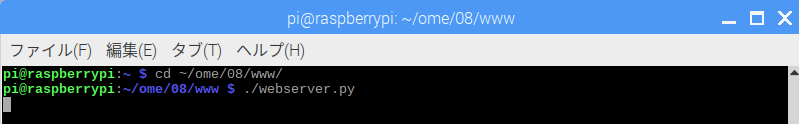
\includegraphics[width=17.006cm]{textbook-img063.png}
\end{center}
アクセスする際は、IPアドレスとともに3000番のポートを指定する必要があります。
起動したディレクトリがドキュメントルート(ウェブページやCGIプログラムから見たルートディレクトリ)になります。

実行した後はこのターミナルではウェブサーバが動いており、メッセージを表示するために使用をします。
\textbf{このターミナルは閉じないでください。}

ウェブページアクセス時のメッセージ例
:

もし、閉じてしまった場合はもう一度起動をしなおしてください。

\begin{center}
	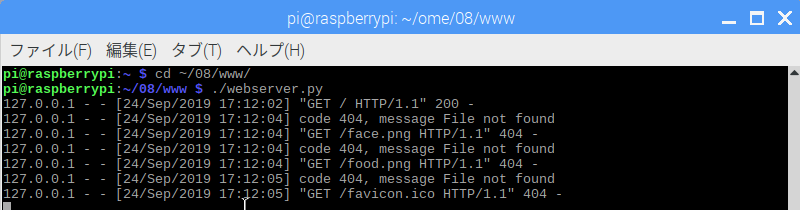
\includegraphics[width=17.006cm]{textbook-img064.png}
\end{center}
HSPのCGIプログラムはサーバー側(ウェブサーバが起動します)もしエラーが発生した場合には、ウェブサーバを起動したターミナルにエラーメッセージが表示されます。
ターミナルを確認してみてください。
エラーが発生したときはCGIプログラムは実行されません。

\begin{center}
	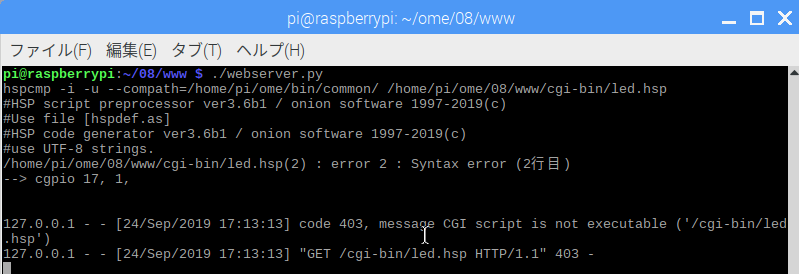
\includegraphics[width=17.006cm]{textbook-img065.png}
\end{center}
{\bfseries ウェブサーバの停止方法}

\ruby{電源}{でんげん}を切る前、ウェブサーバが起動しているターミナルを閉じる前、ウェブサーバを停止したいときは、ウェブサーバを起動したターミナルを選択して

CtrlとCを同時に押します。

\begin{center}
	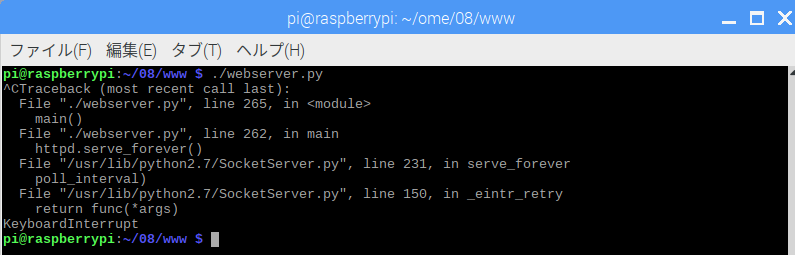
\includegraphics[width=17.006cm]{textbook-img066.png}
\end{center}
これでウェブサーバは終了します。

\section{\ruby{困}{こま}ったら質問フォームから質問しよう!}
質問フォームでは、授業でわからなかったことや確認したいことなどをホームページを通して質問できます。
たくさん質問してわからないことを解決しよう。

1.
ブラウザで\textbf{授業で使うホームページリスト}を開こう。

\textbf{授業で使うホームページリスト}は08フォルダの中のlinks.htmlです

リストの\textbf{子どもIT未来塾質問フォーム}をクリックして開いてくださいFigure~\ref{seq:refFigure0}。

\begin{center}
\begin{minipage}{10.88cm}
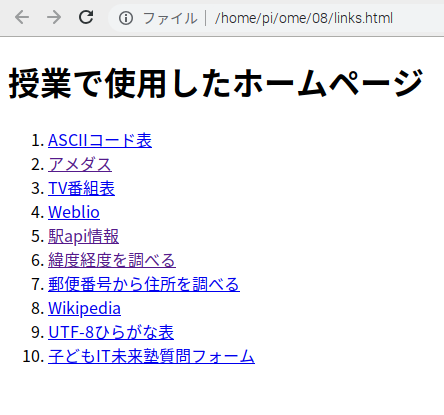
\includegraphics[width=6.638cm]{textbook-img017.png}

Figure {\refstepcounter{Figure}\theFigure\label{seq:refFigure0}}:
ホームページリストより質問フォームを開く
\end{minipage}
\end{center}
{\bfseries スマートフォン等からの場合はhttps://bit.ly/2NHiVgiを開いてください。}

\clearpage
2.
クリックして開くと、質問フォームFigure~\ref{seq:refFigure1}が表示されます

\begin{center}
\begin{minipage}{0.9\textwidth}
{\upshape 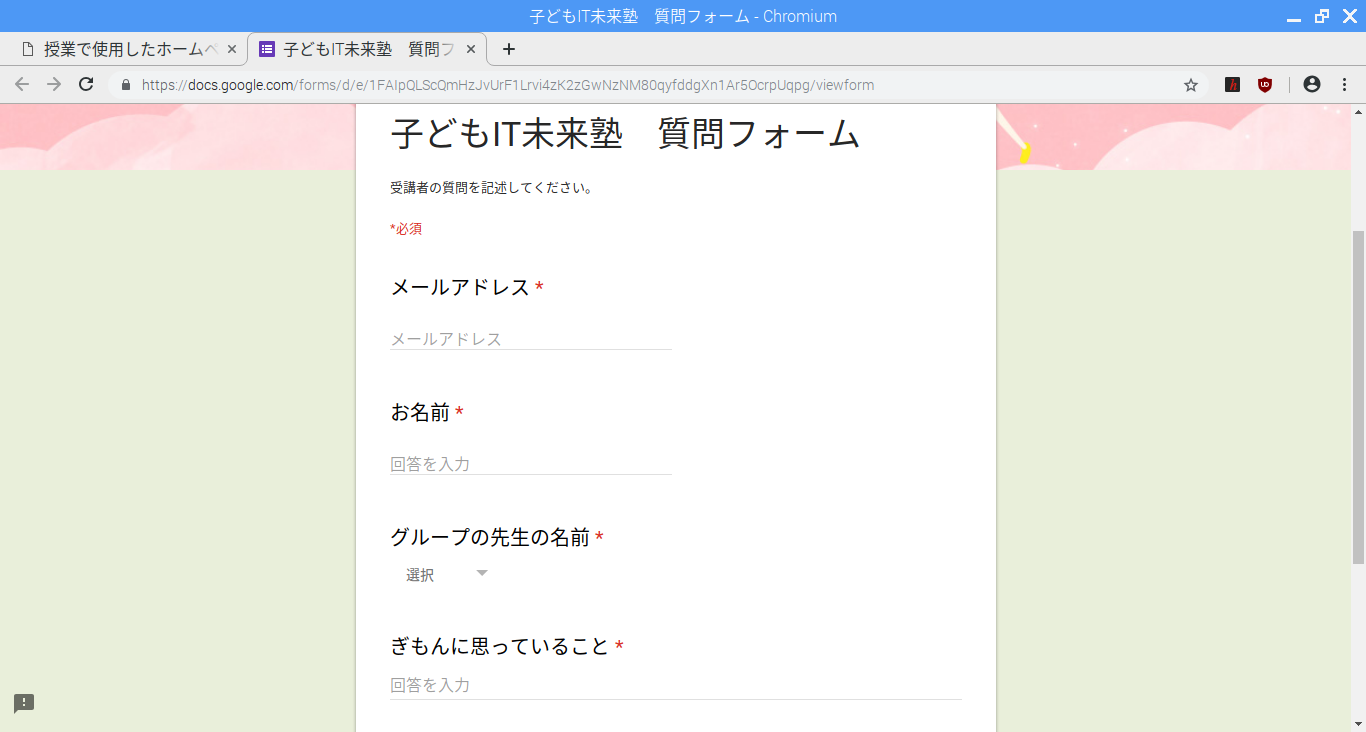
\includegraphics[width=\textwidth]{textbook-img067.png}
\newline
Figure {\refstepcounter{Figure}\theFigure\label{seq:refFigure1}}: 質問フォーム}
\end{minipage}
\end{center}

メールアドレス、お名前、グループの先生の名前、ぎもんに思っていることを入力します。

気軽な質問でもOKです。

例 :

\begin{center}
	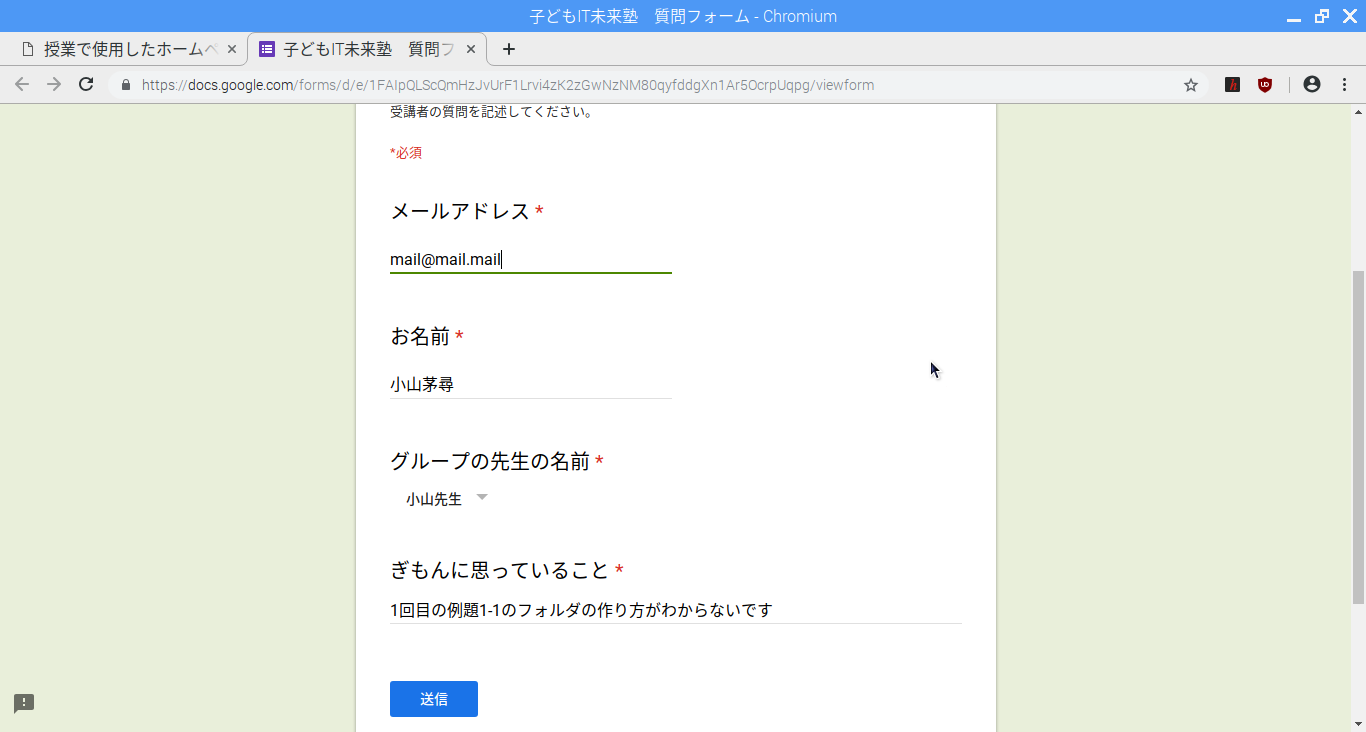
\includegraphics[width=0.9\textwidth]{textbook-img068.png}
\end{center}

\textbf{送信}を押すと質問が送られます。
Figure~\ref{seq:refFigure2}の画面が出たら質問は完了です。

\begin{center}
\begin{minipage}{0.9\textwidth}
{\upshape 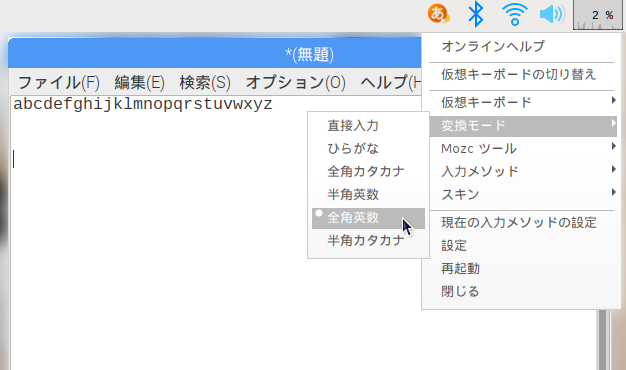
\includegraphics[width=\textwidth]{textbook-img069.png}
 \newline
Figure {\refstepcounter{Figure}\theFigure\label{seq:refFigure2}}: 質問送信画面}
\end{minipage}
\end{center}
メールアドレスのらんに入力したアドレスへグループの先生から回答メールがきます。

{\bfseries \textmd{メールが来るまで、しばらくお待ちください。数日かかる場合があります。}}

\section{\ruby{参考文献}{さんこうぶんけん}}
HeartRails Express https://express.heartrails.com/api.html
